\documentclass[12pt, a4paper]{report}

\usepackage{amsmath}
\usepackage{amssymb}
\usepackage{amsthm}
\usepackage{graphicx}
\usepackage{authblk}
\usepackage{hyperref}
\usepackage{float}

\title{Van-der-Pol Oscillator}
\author{Mrinalgouda Patil}
\affil{Rollno: 130010061}
\date{\today}

\begin{document}
\maketitle

\begin{abstract}
In this work, we present a detailed analysis of the solutions to the equation of Vander-Pol Oscillator. We begin with giving emphasis on the history of how the equation was evolved. Then we look into the numerical analysis or the solutions of the equation. This is followed by the classification of the solutions based on the parameter $\mu$. In the end, we look into the concept of Limit cycles where we show the difference betweent the solutions for larger and smaller values of $\mu$. 
\end{abstract}

\chapter{Introduction}
The Van der Pol equation, name after telecommunications pioneer Balthazar Van der Pol (1889-1959), is a second-order nonlinear differential equation most commonly examined in the field of nonlinear oscillations. Th equation models the oscillating charge of the Van der Pol oscillator, a simple circuit with a parallel capacitor, charge source and inductor in series with a tunnel diode.
\par
The key feature  of the Van der Pol oscillator is that its damping may be positive or negative in relation to the current amplitude of the oscillations. Specifically, larger oscillations are positively damed to become smaller, while smaller oscillations are negatively damped to become larger. all tending toward the same range of dynamic behaviour. In fact, all forms of the unforced Van der Pol oscillator tend toward a single stable limit cycle for their oscillations. For the purposes of telecommunications, circuits providing this functionality are useful in their ability to make both loud and quiet signals more easily perceived by the recipient. The only other equilibrium reached by the Van der Pol equation is the unstable  fixed point with zero amplitude and zero velocity, since a circuit containing no charge or charge source will see no oscillation; however, even the slightest bump of the circuit will eventually create a signal following the expected limit cycle.

\chapter{History}
The Van der Pol oscillator was originally proposed by the Dutch electrical engineer and physicist Balthasar van der Pol while he was working at Philips. Van der Pol found stable oscillations, which he subsequently called relaxation-oscillations and are now known as a type of limit cycle in electrical circuits employing vacuum tubes. When these circuits were driven near the limit cycle, they become entrained, i.e. the driving signal pulls the current along with it. Van der Pol and his colleague, van der Mark, reported in the September 1927 issue of Nature that at certain drive frequencies an irregular noise was deterministic chaos. \cite{Lienard}

The Van der Pol equation has a long history of being used in both the physical and biological sciences. For instance, in biology, Fitzhugh and Nagumo extended the equation in a planar field as a model for action potentials of neurons. The equation has also been utilised in seismology to model the two plates in a geological fault, and in studies of phonation to model the right and left vocal fold oscillators.

\chapter{Dynamics}
In dynamics, the Van der Pol oscillator is a non-conservative oscillator with non-linear damping. It evolves in time according to the second-order differential equation  :

\begin{equation}\
\frac{d^2 x}{dt^2}+\mu(x^2-1)\frac{dx}{dt}+x=0
\end{equation}\\

where x is the position coordinate—which is a function of the time t, and $\mu$ is a scalar parameter indicating the nonlinearity and the strength of the damping.

The equation can be physically construed as an oscillator with a linear spring force and a nonlinear damping force. The following analysis assumes that the factor $\mu >0$. On closer inspection of the equation, it can be seen that when $|x| <1$, the damping force is negative, i.e, reinforces the motion. For $|x| >1$, the damping force is positive and decays the motion. Such behaviour suggests the possibility of an oscillation, in which the system starts at small $x$, is driven to a large $x$ by the amplification, and is then damped back to small $x$.

\section{Numerical Integration}
Let’s write Eq. (1) as a first order system of differential equations,

\[
\begin{bmatrix}
\dot{x} = y \\
\dot{y} = -\mu(x^2-1)\dot{x}-x
\end{bmatrix}
\]

The results of numerical integration of the above equations are presented in the below figures. Numerical integration of these equations shows that every initial condition (except x = 0, ˙x = 0) approaches a unique periodic motion. The nature of this limit cycle is dependent on the value of µ. For small values of µ the motion is nearly sinusoidal, whereas for large values of µ it is a relaxation oscillation, meaning that it tends to resemble a series of step functions, jumping between positive and negative values twice per cycle. Numerical integration shows that the limit cycle is a closed curve enclosing the origin in the x-y phase plane. From the fact that the above equations are invariant under the transformation x $\rightarrow$ -x, y $\rightarrow$ -y, we may conclude that the curve representing the limit cycle is point symmetric about the origin. 

There is also Forced Vander-Pol oscillator where the RHS of the equation is non-zero.
\begin{equation}
\frac{d^2 x}{dt^2}+\mu(x^2-1)\frac{dx}{dt}+x=F
\end{equation}\\
The circuit contains: a triode, a resistor R, a capacitor C, a coupled inductor-set with self inductance L and mutual inductance M. In the serial RLC circuit there is a current i, and towards the triode anode ("plate") a current ia, while there is a voltage ug on the triode control grid. The Van der Pol oscillator is forced by an AC voltage source Es.

\begin{figure}[H]
	\centering
	\begin{tabular} {l}
	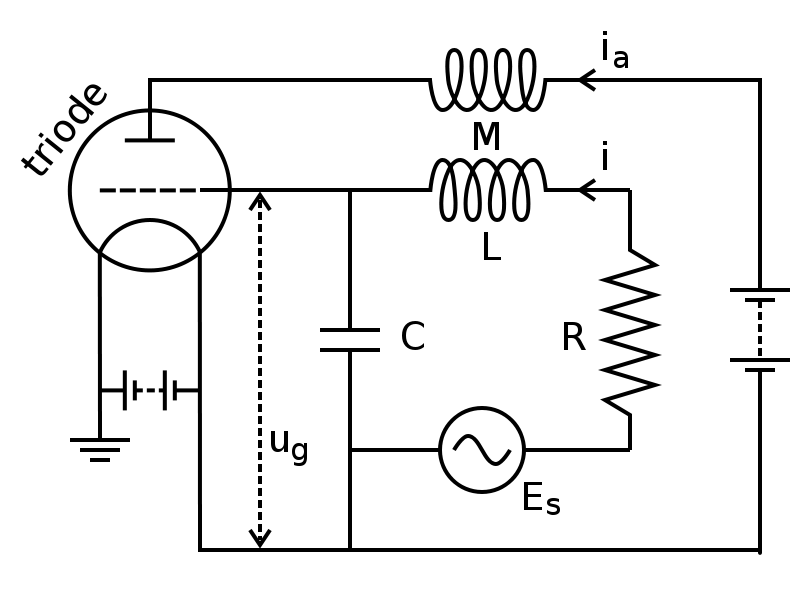
\includegraphics[scale=0.3]{vanderpol.png} 
	\end{tabular}
	\caption{130010061:Electrical circuit involving a triode, resulting in a forced Van der Pol oscillator}
\end{figure}
\label{fig1} 

\chapter{Numerical Solutions}
Lets look at the solution of the equations in detail. In order to clearly understand the solutions for this equation, lets classify the solutions based on the value of $\mu$ by its magnitude.

\section{Small $\mu$}
\subsection{Case 1: $\mu$ = 0.0}


\begin{figure}[H]
	\centering
	\begin{tabular} {l}
	\includegraphics[scale=0.5]{VanderPol_Solutions_mu=0.png} 
	\end{tabular}
	\caption{130010061:Typical solution of van der Pol equation for $\mu$ = 0}
\end{figure}
\label{fig2} 

When $\mu$ = 0, i.e. there is no damping function, the equation becomes: 

\begin{equation}\
\frac{d^2 x}{dt^2}+x=0
\end{equation}

This is a form of the simple harmonic oscillator, and there is always conservation of energy.
The above and the below figures show the variation of solution to the above equation with time.



\section{Large $\mu$}
\subsection{Case 1: $\mu$ = 1.0}
When $\mu$ > 0, the system will enter a limit cycle. Near the origin, 
\begin{equation}
x = \frac{dx}{dt} = 0
\end{equation}\\

the system is unstable, and far from the origin, the system is damped.
The following figure shows the variation of solution to the above equation with time.

\begin{figure}[H]
	\centering
	\begin{tabular} {l}
	\includegraphics[scale=0.5]{VanderPol_Solutions_mu=1.png} 
	\end{tabular}
	\caption{130010061:Typical solution of van der Pol equation for $\mu$ = 1.0}
\end{figure}
\label{fig3} 

\subsection{Case 1: $\mu$ = 5.0}
As described above, for $\mu=5.0$, the system is damped.
The following figure shows the variation of solution to the above equation with time.

\begin{figure}[H]
	\centering
	\begin{tabular} {l}
	\includegraphics[scale=0.5]{VanderPol_Solutions_mu=5.png} 
	\end{tabular}
	\caption{130010061:Typical solution of van der Pol equation for $\mu$ = 5.0}
\end{figure}
\label{fig4} 

\section{Very Large $\mu$}
\subsection{Case 1: $\mu$ = 1000.0}
When $\mu$ > 0, the system will enter a limit cycle. Near the origin, 
\begin{equation}
x = \frac{dx}{dt} = 0
\end{equation}\\

the system is unstable, and far from the origin, the system is damped.
The following figure shows the variation of solution to the above equation with time.

\begin{figure}[H]
	\centering
	\begin{tabular} {l}
	\includegraphics[scale=0.5]{VanderPol_Solutions_mu=1000.png} 
	\end{tabular}
	\caption{130010061:Typical solution of van der Pol equation for $\mu$ = 1000}
\end{figure}
\label{fig5} 

\chapter{The Limit Cycle}
A limit cycle is an isolated close trajectory. This means that its neighbouring trajectories are not closed – they spiral either towards or away from the limit cycle. Thus, limit cycles can only occur in nonlinear systems. A stable limit cycle is one which attracts all
neighbouring trajectories. A system with a stable limit cycle can exhibit self-sustained oscillations – most of the biological processes of interest are of this kind.

The solution to the Van-der-Pol equation can be depicted using Limit cycles. These limit cycles are different for smaller and higher values of $\mu$. 

\begin{figure}[H]
	\centering
	\begin{tabular} {l}
	\includegraphics[scale=0.5]{Limit_cycle_mu=0.png} 
	\end{tabular}
	\caption{130010061:Solution of van der Pol equation for small values of $\mu$}
\end{figure}
\label{fig6} 

\begin{figure}[H]
	\centering
	\begin{tabular} {l}
	\includegraphics[scale=0.5]{Limit_cycle_mu=3.png} 
	\end{tabular}
	\caption{130010061:Solution of van der Pol equation for large values of $\mu$}
\end{figure}
\label{fig7}

Combining the above two plots, we get the below image which shows the limit cycles for various  $\mu$'s.\cite{belur}
\begin{figure}[H]
	\centering
	\begin{tabular} {l}
	\includegraphics[scale=0.5]{all_in_one.png} 
	\end{tabular}
	\caption{130010061:Solution of van der Pol equation for large values of $\mu$}
\end{figure}
\label{fig8}

\chapter{Source Code}
\begin{itemize}
\item Public git repository with open source code can be found at \url{https://github.com/mpcsdspa/sdesproject1}
\item Python 2.7 version is required to run the Python code
\item Numpy with version 1.8.2 or higer is required
\item Matplotlib with version 1.3.1 or higher is required
\item Scipy module needs to be installed in the system
\item Ipython notebook or Jupyter notebook is required for perusing the ipynb file
\item The system must have the ffmpeg installed for watching the animation in Ipython notebook
\end{itemize}

%\bibliography{bib_file}{}
%\bibliographystyle{plain}
\bibliographystyle{plain}
\bibliography{Ref}


\end{document}
